\documentclass[border=5pt]{standalone}
\usepackage{tikz}
\begin{document}
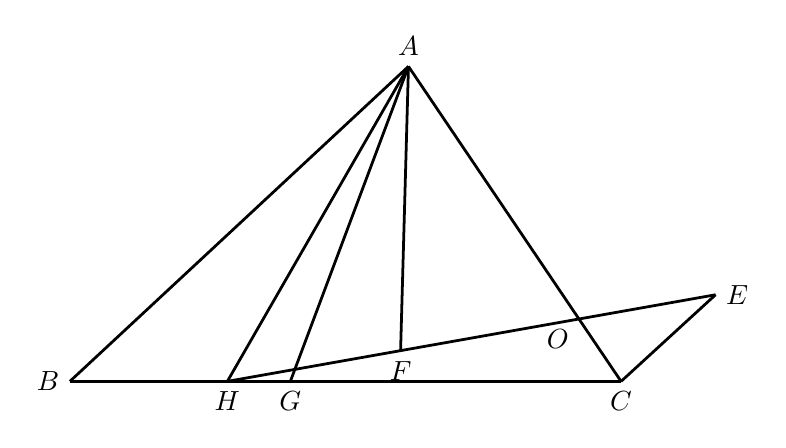
\begin{tikzpicture}[line width=1pt]
  % coordinates
  \coordinate (B) at (0,0);
  \coordinate (C) at (7,0);
  \coordinate (A) at (4.3,4);
  \coordinate (D) at (2,0);
  \coordinate (G) at (2.8,0);
  \coordinate (E) at (8.2,1.1);
  \coordinate (F) at (4.2,0.39);
  \coordinate (O) at (6.47,0.79);
  % lines
  \draw (B) -- (C);
  \draw (A) -- (B);
  \draw (A) -- (C);
  \draw (A) -- (D);
  \draw (A) -- (G);
  \draw (A) -- (F);
  \draw (D) -- (E);
  \draw (C) -- (E);
  % labels
  \node[above] at (A) {$A$};
  \node[left] at (B) {$B$};
  \node[below] at (C) {$C$};
  \node[below] at (D) {$H$};
  \node[below] at (G) {$G$};
  \node[below] at (F) {$F$};
  \node[below left] at (O) {$O$};
  \node[right] at (E) {$E$};
\end{tikzpicture}
\end{document}
